
\documentclass{cccg16}

\usepackage{amssymb, amsmath}
\usepackage{graphicx}
\usepackage{hyperref}
\usepackage[utf8]{inputenc}
\usepackage[T1]{fontenc}
\usepackage{lmodern}
\usepackage{hhline}
\usepackage{wrapfig}
\usepackage{subfig}
\usepackage{listings}
\usepackage{courier}
\usepackage{float}
\usepackage{color}
\usepackage{dcolumn}

\usepackage{lipsum}

\DeclareMathOperator{\sign}{sign}
\DeclareMathOperator{\fma}{fma}
\DeclareMathOperator{\round}{round}
\def\Jack#1{{\bf [[#1]]}\ignorespaces}
\def\Michael#1{{\bf \color{red} [[#1]]}\ignorespaces}
%\def\Jack#1{\ignorespaces}%% uncomment to hide remarks
%\def\Michael#1{\ignorespaces}%% uncomment to hide remarks

\lstset{basicstyle=\ttfamily}

\title{On the Precision to Sort Line-Quadric Intersections}
\author{Michael Deakin \and Jack Snoeyink\thanks{School of Computer
    Science, University of North Carolina at Chapel Hill, {\tt
      mfdeakin@cs.unc.edu}, {\tt snoeyink@cs.unc.edu}}}

\index{Deakin, Michael}
\index{Snoeyink, Jack}

\newcolumntype{d}[1]{D{.}{\cdot}{#1} }

\begin{document}
\thispagestyle{empty}
\maketitle

\begin{abstract}
  To support exactly tracking a neutron moving along a given line
  segment through a CAD model with quadric surfaces, this paper
  considers the arithmetic precision required to compute the order of
  intersection points of two quadrics along the line segment. When the
  orders of all but one pair of intersections are known, we show that a
  resultant can resolve the order of the remaining paiir using only
  half the precision that may be required to eliminate radicals by
  repeated squaring. We compare the time and accuracy of our technique
  with converting to extended precision to calculate roots.
\end{abstract}


\section{Introduction}
In this work, we are concerned with ordering the points of
line-quadric intersections in 3 dimensions, where the inputs are
representable exactly using $w$-bit fixed-point numbers.  We will
actually use floating point in storage and computation, but our
guarantees will be for well-scaled inputs, which are easiest described
as fixed-point.  A {\it representable point}~$q$ or {\it representable
  vector}~$v$ is a $3$-tuple of representable numbers $(x, y, z)$. The
line segment from point~$q$ to~$q+v$ is defined parametrically for
$t\in [0,1]$ as $\ell(t)=q+tv$; note that there may be no
representable points on line $\ell$ except its endpoints (and even
$q+v$ may not be representable, if the addition carries to
$w+1$~bits.)

A quadratic is an implicit surface defined by its 10 representable coefficients,
\begin{align*}Q(x, y, z)=q_{xx} x^2 &+ q_{xy} xy + q_{xz} xz + q_x x + \dots \\
&+ q_{zz} z^2 + q_{z} z + q_c = 0.
\end{align*}
For more accuracy, we can allow more precision for the linear and
quadratic coefficients, since we will need $3w$~bits to exactly
multiply out the quadratic terms, or we can use a representable
symmetric $3{\times} 3$ matrix~$M$, a representable vector~$v$, and a
$3w$-bit constant~$R$ to give a different set of quadrics $\tilde Q(p)
= (p-v)^TM(p-v) = R$ that is closed under representable translations
of~$v$. Whichever definition of quadrics is chosen, the parameter
values for line-quadric intersections are the roots of $Q(\ell(t))=0$,
which can be expressed as a quadratic $at^2+2bt+c=0$ whose
coefficients can have at most $3w+4$~bits.  (Four carry bits suffice
to sum the $3w$-bit products; $w=16$ allows exact coefficient
computation as IEEE 754 doubles; $w=33$ as pairs of doubles.)

These definitions are motivated by a problem from David Griesheimer,
of Bettis Labs: rather than tracking a particle through quadric
surfaces in a CAD model, would it be more robust to compute the
intervals of intersections with a segement?  We compare three methods
to order line-quadric intersections.  Our methods, particularly the
third, are  developed and tested for the case where only
one pair of roots has a difference that is potentially overwhelmed by
the rounding errors in the computation. We comment at the end how to
handle pairs of quadric surfaces that have more than one pair of
ambiguous roots.


\section{Methods}
This section outlines three methods---Approximate Comparison, Repeated
Squaring, and Resultant---to sort the intersections with two quadrics,
$Q_1$ and $Q_2$, with a given line $\ell(t)$, or equivalently, the
roots of two quadratics, $a_1t^2+2b_1t+c_1=0$ and
$a_2t^2+2b_2t+c_2=0$.  For each, we evaluate correctness, precision,
and floating-point arithmetic operations (FLOPs) required.

\subsection{Approximate Comparison}
The approximate comparison method computes, for $i\in\{1, 2\}$, the
roots~$r_i^\pm=({b_i\pm\sqrt{b_i^2-a_ic_i}})/{a_i}$ approximately by
computing each operation in IEEE 754 double precision or in extended
precision.  Actually, to avoid subtractive cancellation, we calculate
one of the two roots as $r_i^{-\sign
  b_i}=-c_i/({b_i+(\sign{b_i})\sqrt{b_i^2-a_ic_i}})$.  The order of
any two chosen approximate roots can be calculated exactly
as~$\sign(r_1^\pm-r_2^\pm)$.

The rounding of floating point arithmetic means that even with
representable input, the correct order is not guaranteed unless we
establish a gap or separation theorem (which are also established
using resultants~\cite{brownawell2009lower,emiris2010dmm}) and compute with sufficient
precision.  Without a guarantee, this method requires very little
computation.  Computing both roots takes $12$ FLOPs, with one more to
compute the sign of the difference.  Moreover, the roots can be reused
in a scene of many quadrics.

We also use extended precision, where the multiplications and addition
in the discriminants are calculated with $6w$ bits, square root and
addition at $12w$ bits, and divisions at $24w$ bits.  To actually
perform the comparison, one final subtraction is required at 24 times
the initial precision -- 1 FLOP, with an initialization cost of 10
FLOPs per quadric intersecting the line.

\subsection{Repeated Squaring}
The repeated squaring method computes $\sign(r_1^\pm-r_2^\pm)$ by
algebraic manipulations to eliminate division and square root
operations, leaving multiplications and additions whose precision
requirements can be bounded.  It uses, for $x\ne 0$, the property that
$\sign(y)=\sign(x)\sign(x\cdot y)$.  Divisions can be removed
directly, since $\sign(r_1^\pm-r_2^\pm)=\sign(a_1 a_2)\sign(a_1 a_2
(r_1^\pm-r_2^\pm))$.  One square root can be eliminated by multiplying
by $r_1^\pm-r_2^\mp$, giving~$\sign(a_1 a_2)\sign(a_1 a_2
(r_1^\pm-r_2^\mp))\cdot\sign(a_1^2 a_2^2 (r_1^\pm - r_2^\pm) (r_1^\pm
- r_2^\mp))$.  When simplified, the final sign is computed
from~$a_2^2b_1^2-2a_1a_2^2c_1+2a_1^2a_2c_2-a_1a_2b_1b_2\pm
\sqrt{(a_1a_2b_2-a_2^2b_1)^2(b_1^2-4a_1c_1)}$.

The expression under the radical is correctly computed with $8\times$
the input precision; the remaining expression can be evaluated to a
little more than $4\times$ input precision in floating point, or can
be evaluated in fixed point in $8\times$ input precision by isolating
the radical and squaring one last time.

This method not only requires high precision, but also a large number
of FLOPs.  Computing the unambiguous sign of the difference of the
roots requires 15 FLOPs total, and correctly computing the final sign
requires another 24 FLOPs.  Unfortunately, many of the computed terms
require coefficients from both polynomials; only the discriminants,
squares, and products can precomputed, which reduces the number of
FLOPs by 14.  This brings us to 25 FLOPs per comparison, with an
initialization cost of 14 FLOPs per quadric.

Note that this method uses our assumption that we know
$\sign(r_1^\pm-r_2^\mp)$ when computing $\sign(r_1^\pm-r_2^\pm)$, but
we can learn this from a lower precision test against $-b_2/a_2$,
since $r_2^- \le -b_2/a_2 \le r_2^+$.

\begin{equation}
  res(P, Q)=\begin{pmatrix}
    p_m & \dots & & p_0 & 0 & & 0\\
    0 & p_m & \dots & & p_0 & & 0\\
    & \ddots & & & & \ddots\\
    0 & 0 & & p_m & \dots & & p_0\\
    q_n & \dots & & q_0 & 0 & & 0\\
    0 & q_n & \dots & & q_0 & & 0\\
    & \ddots & & & & \ddots\\
    0 & & q_n & \dots & & q_0\\
  \end{pmatrix}
  \label{eq:sylv}
\end{equation}

\subsection{Resultant}
The resultant method computes the order of two intersections from the
resultant for their polynomials, which can be written as the
determinant of their Sylvester Matrix~\cite[Section~3.5]{cheeyap}.
The general Sylvester Matrix for polynomials~$P(t)=p_m t^m + \dots +
p_0$ and~$Q(t)=q_n t^n + \dots + q_0$ is defined as in Equation
\ref{eq:sylv}.
The resultant is also the product of the differences of $P$'s roots,
$a_1$, \dots, $a_n$, and $Q$'s roots, $b_1$, \dots, $b_m$, as in
Equation~\ref{eq:resultant}.~\cite[Section~6.4]{cheeyap}
\begin{equation}
  res(P, Q)=p_m^n q_n^m \prod_{i=1}^m\prod_{j=1}^n (a_i-b_j)
  \label{eq:resultant}
\end{equation}

\begin{figure*}
  \begin{align}
    \sign(a_1-b_1)=\sign(res(P, Q))\sign(p_m^n)\sign(q_n^m)
    \prod_{i=2}^m\prod_{j=2}^n[\sign(a_i-b_j)\sign(a_1-b_j)\sign(a_i-b_1)]
    \label{eq:signroot}
  \end{align}
\end{figure*}

The two expressions for the resultant provide us with another method
of computing the sign of one of the differences of the two roots.
Under our assumption that we know the order of all pairs or roots
except, say, $a_1$ and $b_1$, we can compute $\sign(a_1-b_1)$ from the
determinant and known signs, as in Equation \ref{eq:signroot} at the top of the next page.  The
signs need not be multiplied; we simply count the negatives.  With
quadratics, $m=n=2$, so the signs of the leading ~$p_2^2$ and~$q_2^2$
will be positive and can be ignored.

The determinant can be computed with half the precision and fewer
floating point operations than repeated squaring to correctly compute
the sign of the differences of roots of the polynomials.

Computing a general $4{\times} 4$ determinant takes about 120
multiplications, and computing the determinant of the Sylvester matrix
itself would naively take~$35$ FLOPs for each comparison.  We can do better in Equation~\ref{eq:sylvpoly} by writing
the determinant in terms of the discriminants and other
precomputed $2{\times} 2$ minors from each polynomial.  This brings us to 11 FLOPs per comparison, with an
initialization cost of 7 FLOPs per intersection.

\begin{figure*}
  \begin{equation*}
    \Delta=\begin{vmatrix}
    a_1 & b_1 & c_1 & 0\\
    0 & a_1 & b_1 & c_1\\
    a_2 & b_2 & c_2 & 0\\
    0 & a_2 & b_2 & c_2\\
    \end{vmatrix}=
    a_1^2 c_2^2 + c_1^2 a_2^2 + b_1^2 a_2 c_2 + b_2^2 a_1 c_1 -
    b_1 c_1 a_2 b_2 - a_1 b_1 b_2 c_2 - 2 a_1 c_1 a_2 c_2
  \end{equation*}
  \begin{align}
    \alpha_i=a_i^2,\,\, \gamma_i=c_i^2,\,\,
    \delta_i=a_i b_i,\,\, \epsilon_i=a_i c_i,\,\, \zeta_i=b_i c_i,\,\,
    D_i=b_i^2-\epsilon_i,\,\,
    i\in {1, 2}\\
    \Delta = \alpha_1 \gamma_2 + \gamma_1 \alpha_2 +
    D_1 \epsilon_2 + \epsilon_1 D_2 - \zeta_1 \delta_2 -
    \delta_1 \zeta_2
  \label{eq:sylvpoly}
  \end{align}
\end{figure*}

\section{Experimental Evaluation}
We experimentally evaluated  the  resultant method  and the  approximate computation method with both machine
precision and extended precision.  Repeated Squaring is dominated by the other methods so was not tested.

We created two types of test scenes that had touching surfaces so that
random lines migh have some chance (albeit small) to give incorrect
orders under approximation, and count the number of disagreements.  We
evaluated time per comparison for each method on computers with
different processors.  Finally, by varying tne number of surfaces in
the second type of scene, we could use linear regression to determine
the contribution to running time from per quadric and per comparison
terms.
 

\subsection{Experimental Setup}
All methods were implemented in C++, and were tested by computing the
line-quadric intersection orders along 100k lines, created from pairs
of uniformly random points with single precision coordinates, in
scenes of quadric surfaces, whose creation is described in the next
subsection.  Machine precision tests were performed in IEEE 754, with
quadratic coefficients and discriminants stored as floats, even though
automatic promotion performed intermediate computations as doubles.
MPFR\cite{mpfr} was used to support arbitrary precision in both the
approximate comparison and the resultant methods.

The first step of the evaluation for a line $\ell$ and quadric $Q$ was
to determined if there was a real intersection by evaluating the
discriminant of the quadratic~$p(t)=Q(\ell(t))$.  This evaluation was
done in machine precision, so there is a small chance that near
tangent intersections may have been missed due to numeric error in
calculating the discriminant. (In our application, missing near
tangent intersections was allowed, but getting orders wrong had been
known to trap particles into repeatedly trying to cross the same pair
of surfaces, which tends to worry a physicist.)

If the intersections are deemed to exist, the second step is to
compute the roots at machine precision.  These roots are needed to
determine if the order of a pair of intersections is ambiguous or not.
Finally, the stl sort algorithm is used to sort the intersections.

The comparison function used for sorting came from the method being
evaluated.  The machine precision approximate comparison just returns
the difference of the previously computed roots.  In the increased
precision approximation and the resultant method, the difference of
the roots is compared against a threshold.  If the difference was
smaller than a threshold of $2^{-15}$, the more accurate method
provided is used to determine the order, and an appropriate value is
returned.  This occured infrequently for a random line, 

\Jack{Timing measurments were taken by  ?? (Say what function you used for timing, because some clocks have pretty coarse granularity.}

We ran tests on two computers with different speeds and operating
systems; we name them by their operating systems.

\noindent{\bf Arch} was a Core i3 M370 processor with 2 cores, a 3 MB
cache, and 4 GB of DDR3 memory clocked at 1 GHz.  It ran an up-to-date
installation of Arch Linux, kernel version 4.4, and GCC 6.0 was used
to compile the code.  For the tests, the performance manager was set
to keep the CPU clock at 2.4 GHz, and the process was run with a nice
value of $-20$.

\noindent{\bf Gentoo} was a Core 2 Duo E6550 processor with two cores,
a 4 MB cache, and 8 GB of DDR2 memory clocked at 667 MHz.  It ran an
up-to-date installation of Gentoo Linux, kernel version 4.1 and GCC
4.9 was used to compile the code.  For the tests, the performance
manager was set to keep the CPU clock at 2.3 GHz, with a nice value of
$-20$.

A Geekbench benchmark was employed to estimate the floating point
processor speeds, Arch 1702, and Gentoo 1408. Thus, on average, Arch
was capable of about 1.2 times more FLOPS than the Gentoo computer.


\subsection{Test Scenes}
We created two types of test scenes: a single scene of Packed Spheres
and and a set of scenes of Nested Spheres.  The test scenes consisted
of quadric surfaces stored as IEEE754 single precision floating point
numbers.  We preferred spheres and ellipsoids, since any intersecting
line would intersect twice, possibly with a repeated root.  Sorting
isolated single roots is easier, since, for example, the intersection
with a plane requires less precision. The quadric surfaces were
constructed from the unit cube that has one corner at the origin and
the opposite corner at $(1.0, 1.0, 1.0)$.

The one scene of Packed Spheres consisted of 1331 spheres in a
hexagonal close packing lattice shown in Fig.~\ref{fig:testScenes}.
This ensures that the spheres each have 12 intersecting or nearly
intersecting neighbors.  The spheres each have a radius of
about~$0.05$ units, and are spaced about~$0.05$ units from each other.
The initial sphere is centered at the origin, and one of the axes of
the lattice is aligned with the $y$ axis of the coordinate frame.  The
coefficients of the spheres are scaled so that the coefficients of the
squared terms were all $1.0$. This caused the exponent range for the
non-zero coefficients of the spheres to be between~$-8$ and~$1$.

We used eleven scenes of Nested Spheres. One, shown in
Fig.~\ref{fig:testScenes}, had $n=10$ spheres, the others had
$n=100i$, for $1\leq i \leq 10$.  The first sphere was centered
at~$x_0=0.5, y_0=0.5, z_0=0.5$ units with a radius of~$R_0=0.5$ units.
The radius of successive spheres decreased linearly so that the final
sphere's radius was $R_n=2^{-16}$ units.  Thus,
$R_i=R_{i-1}-(R_0-R_n)/n$.  The $x$ position of successive spheres
increased linearly to fix the minimum distance at~$\epsilon=2^{-19}$
units. Thus, $x_i=x_{i-1}+(R_0-R_n)/n-\epsilon$.  The exponent range
for the non-zero coefficients of the spheres was chosen to be
between~$-1$ and~$0$.

\begin{figure}
  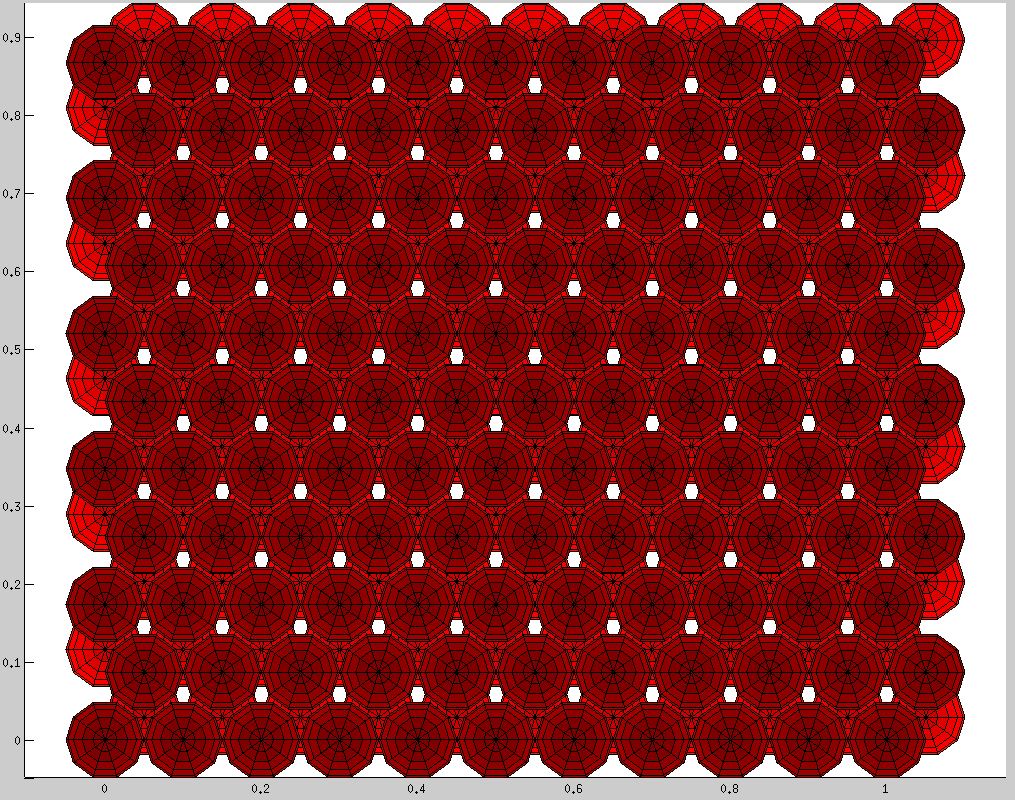
\includegraphics[width=0.5\textwidth]{imgs/packedSpheres.png}
  \vspace{5mm}
  
  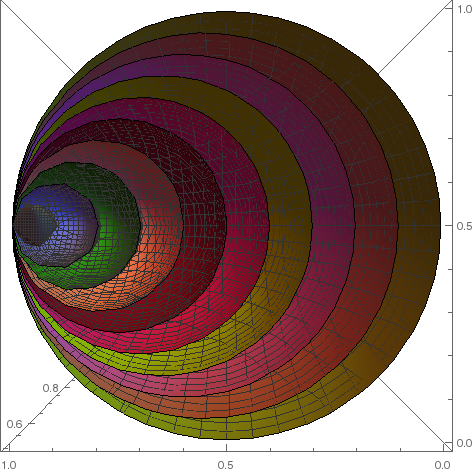
\includegraphics[width=0.5\textwidth]{imgs/hardEllipsoidsSingle.png}
  \caption{Test Scenes of 1331 Packed Spheres and 10 Nested Spheres,
    which is smallest of a family of eleven.  Random lines in Packed
    Spheres have some chance of being near sphere contacts.  Random
    lines in Nested Spheres are unlikely to, unless they are biased to
    pass by the near tangency.}
  \label{fig:testScenes}
\end{figure}

\subsection{Analysis}
To analyze the results, we computed the least squares linear fit of
the timing data.  For the Packed Spheres, we used the number of
comparisons made as our independent variable, and computed a linear
coefficient for it along with a constant term.  For the Nested Spheres
set of scenes, we aggregated the test results for the scenes so we
could fit the line to two independent variables; the number of
comparisons made, and the number of quadric surfaces in the scene.
Fitting the time it takes to make a comparison to a linear
relationship makes sense, as the bulk of the sorting time is taken up
by performing these comparisons.  It also makes sense for the time to
be linearly related to the number of quadrics in the scene, as the
cached values are only computed once for each quadric, and are likely
to significantly affect the time a comparison takes.

\section{Experimental Results}
The results of the experiments are shown in Table \ref{tab:times}.
Each method took approximately the same amount of time to process each
quadric, though the resultant method consistently took the longest.
This is because the resultant method caches some of the intermediate
values when the first comparison is made, shifting some portion of the
cost from the ms/Comp term to the ms/Quadric term.  The
amount that is shifted is determined by how many quadrics a random
line can be expected to intersect, and how many ambiguous orderings a
single line-quadric intersection will be involved in.  The increased
precision approximation method also took longer than the machine
precision approximation method for essentially the same reason as the
resultant method.  It's not entirely clear why it took less time than
the resultant method, as it performs harder computations on the first
use of the quadrics roots than the resultant.

The second term is approximately how much time each comparison takes.
Not surprisingly, the machine precision method took very little time
per comparison.  This is because nearly all of it's work is done on a
per quadric basis - the roots are calculated for each quadric once,
and only a subtraction is required for each comparison. The resultant
method also performed significantly better than the increased
precision method on a per comparison basis.  This is as expected,
given the reduction in the amount of precision, the number of FLOPs
required, and the lack of operations such as square roots and
divisions.

The constant term appears to be rather meaningless when we measure the
ms/Quadric term.  This is good, because it shows that when the
ms/Quadric term is not measured, that is mainly what the constant term
consists of.  Thus, we expect and observe the same results as in the
ms/Quadric term.  This gives confidence there that we are not missing other major terms
that should be considered.

\begin{figure}
  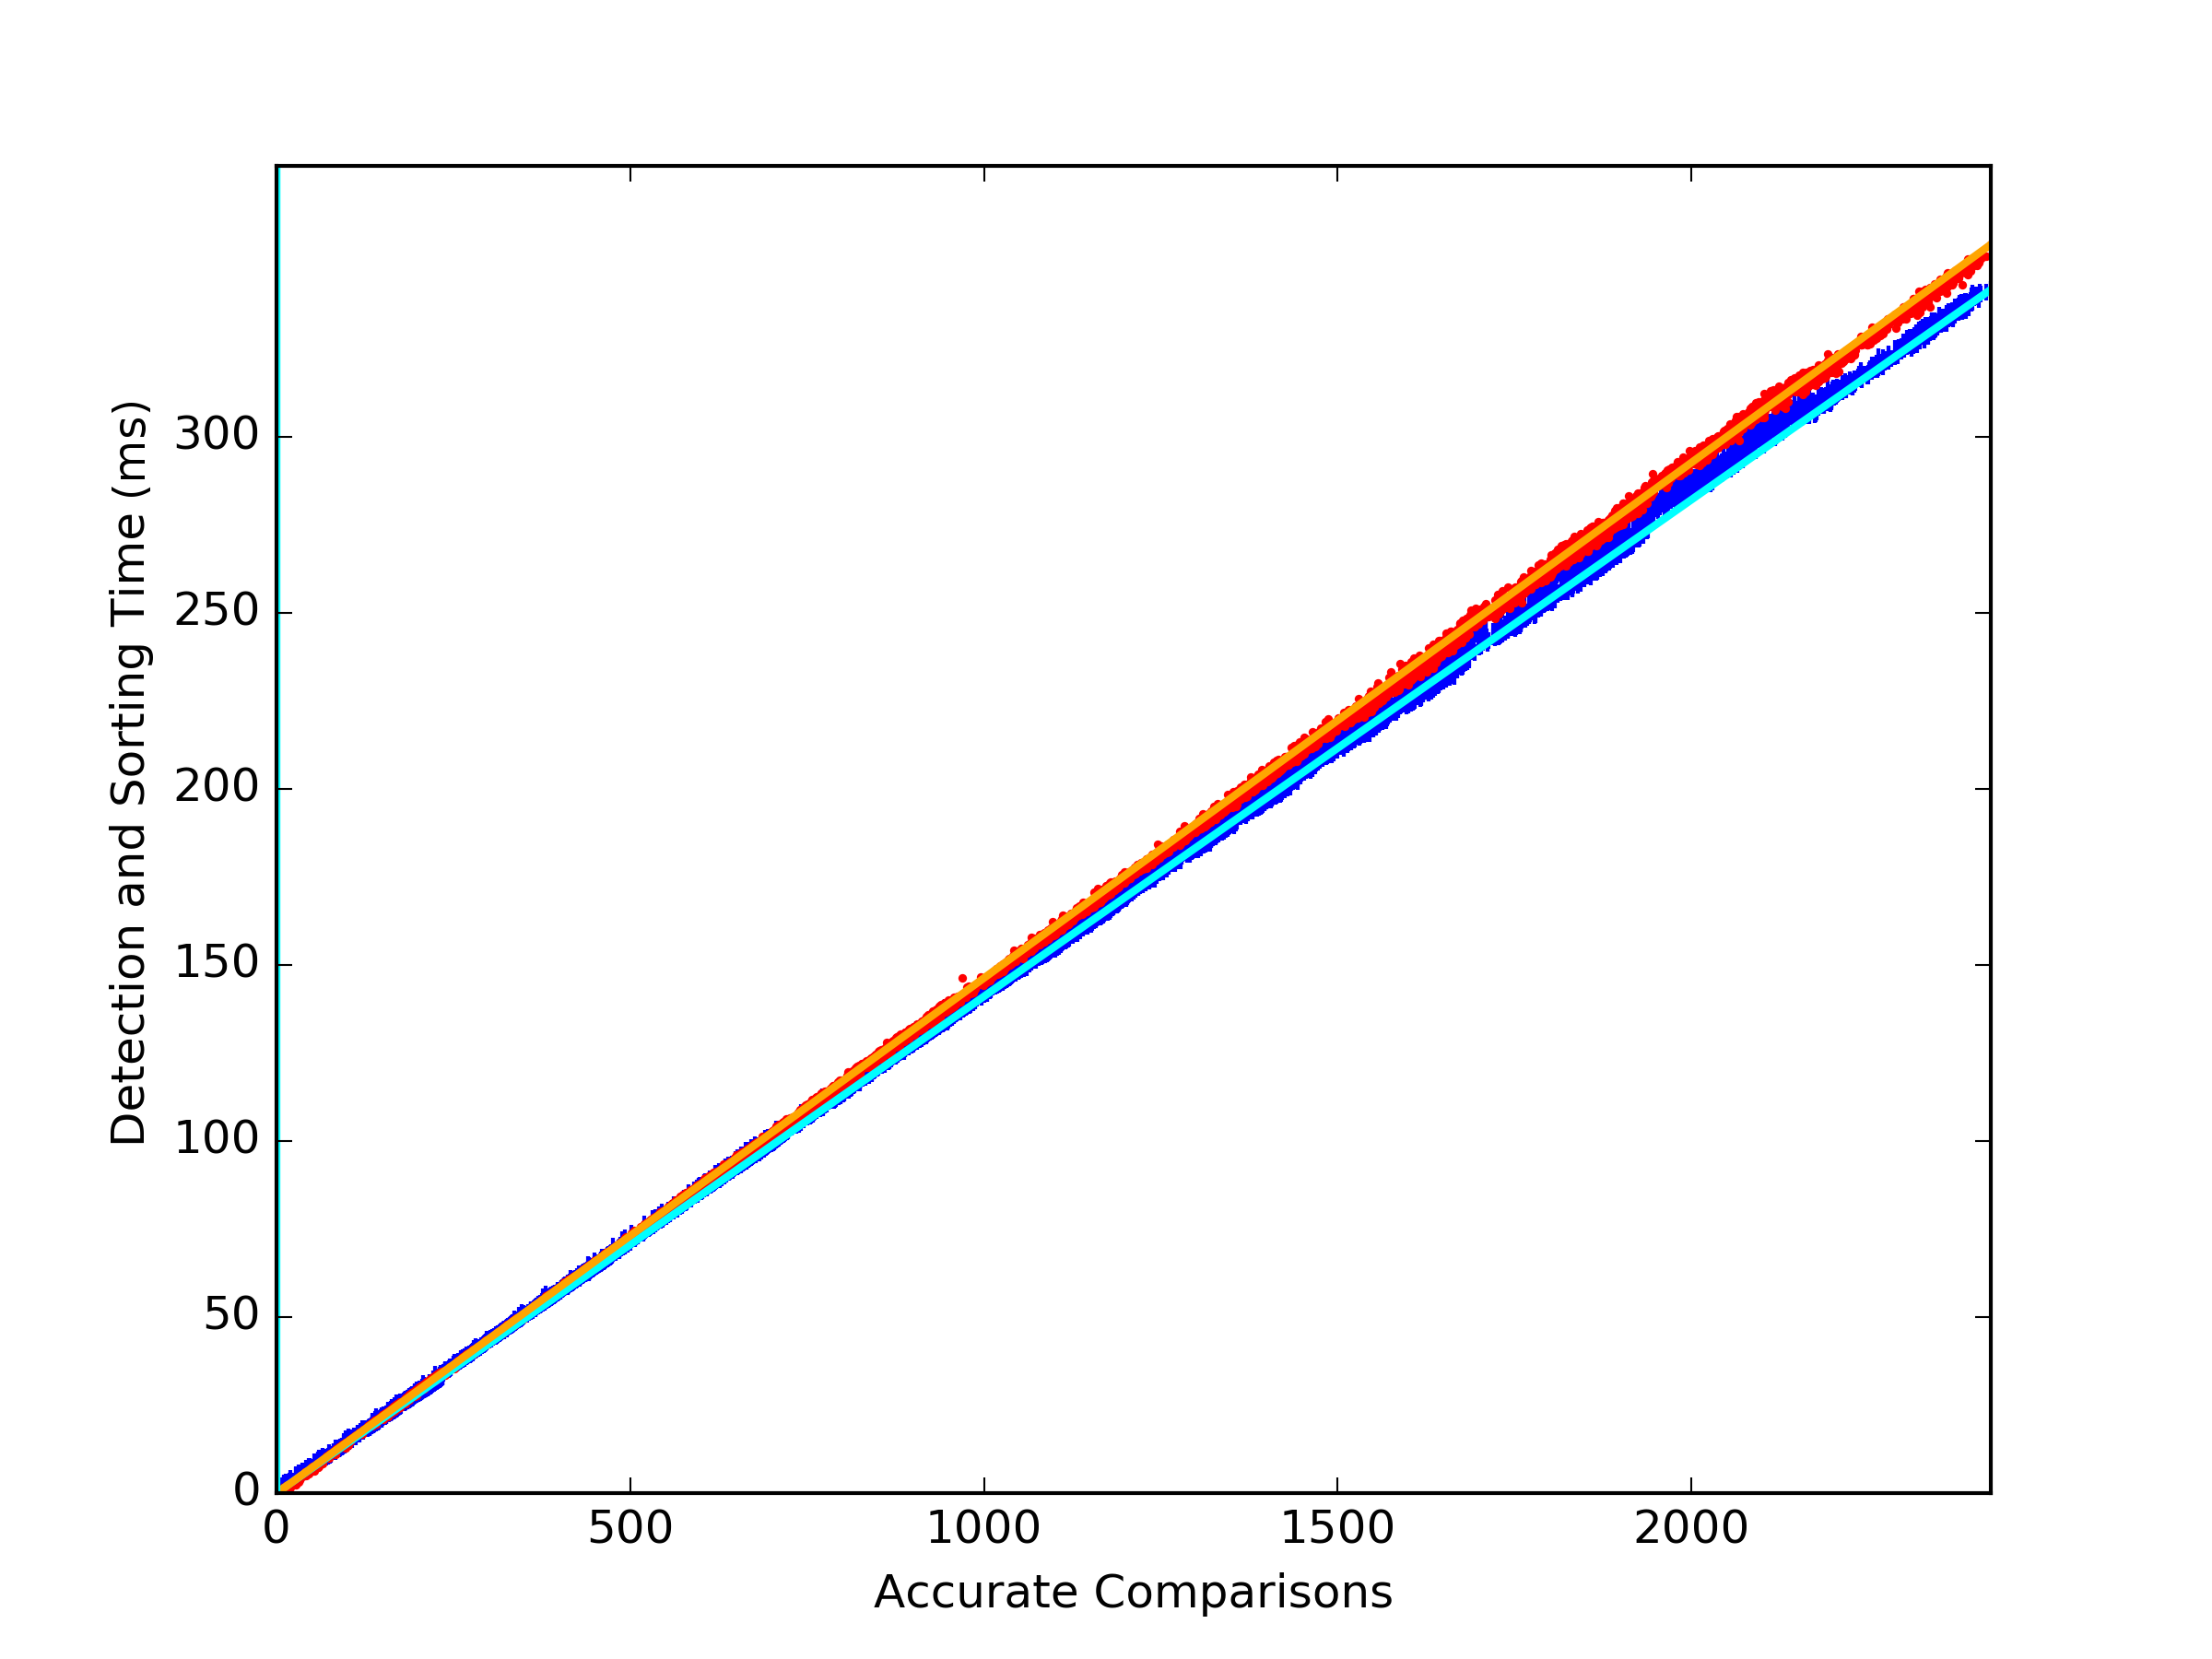
\includegraphics[width=0.55\textwidth]{imgs/hardEllipsoidsSingle_gentoo_adjusted.png}
  \caption{Evaluation Time for a Line (ms) vs. the Number of
    Comparisons; 100k lines sorting on the Gentoo machine; {\bf Green:
      Approximation Method at Input Precision}; {\bf Red:
      Approximation Method at $24\times$ the Input Precision}; {\bf
      Blue: Resultant Method}}
  \label{fig:linefit}
\end{figure}

Figure \ref{fig:linefit} shows a plot of the results from one of the
tests.  It appears to confirm our expectation that the time required
is linearly coorelated with the number of precision increases.

\begin{table*}
  \caption{Timing Results of the Approximate Comparison and Resultant
    Comparison, 100k lines in the Packed Spheres test, 1100k lines in
    the set of 11 Nested Spheres tests}
  \label{tab:times}
  \begin{tabular}{|l|l|ll|lll|l|}
\hline
Machine & Scene & Method & Disagreements & $\frac{\text{ms}}{\text{Quadric}}$ & $\frac{\text{ms}}{\text{Comparison}}$ & Constant $\text{ms}$ & Residual ($\text{ms}^2$)\\
\hhline{|=|=|==|===|=|}
Ubuntu & Packed & Increased Prec. & \hphantom{1}--- & -- & \hphantom{-}0.06823 & \hphantom{-}5.399 & \hphantom{10}1194.8288\\
& Spheres & Approximate & 103 & -- & -0.009685 & \hphantom{-}5.399 & \hphantom{10}1161.2192\\
&& Resultant & \hphantom{1}89 & -- & \hphantom{-}0.05687 & \hphantom{-}5.408 & \hphantom{10}1194.1208\\
\hline
& Nested & Increased Prec. & \hphantom{1}--- & 0.004163 & \hphantom{-}0.07064 & -0.002835 & \hphantom{1}28554.479\\
& Spheres & Approximate & \hphantom{1}13 & 0.004098 & \hphantom{-}0.000255 & -0.001070 & \hphantom{10}2806.9520\\
&& Resultant & \hphantom{10}0 & 0.004309 & \hphantom{-}0.05846 & \hphantom{-}0.007079 & \hphantom{1}32989.590\\
\hline
Arch & Packed & Increased Prec. & \hphantom{1}--- & -- & \hphantom{-}0.1364 & \hphantom{-}4.893 & \hphantom{100}334.98312\\
& Spheres & Approximate & \hphantom{1}85 & -- & \hphantom{-}0.000304 & \hphantom{-}4.942 & \hphantom{100}316.04740\\
&& Resultant & \hphantom{1}75 & -- & \hphantom{-}0.1139 & \hphantom{-}4.921 & \hphantom{100}327.24112\\
\hline
& Nested & Increased Prec. & \hphantom{1}--- & 0.003835 & \hphantom{-}0.1157 & \hphantom{-}0.05856 & 582387.69\\
& Spheres & Approximate & \hphantom{1}11 & 0.003864 & \hphantom{-}0.000591 & -0.01970 & \hphantom{10}7533.7867\\
&& Resultant & \hphantom{10}1 & 0.004088 & \hphantom{-}0.09580 & \hphantom{-}0.05074 & 558251.79\\
\hline
Gentoo & Packed & Increased Prec. & \hphantom{1}--- & -- & \hphantom{-}0.1711 & \hphantom{-}4.522 & \hphantom{100}255.93646\\
& Spheres & Approximate & \hphantom{1}94 & -- & \hphantom{-}0.004651 & \hphantom{-}4.513 & \hphantom{100}256.48723\\
&& Resultant & \hphantom{1}84 & -- & \hphantom{-}0.1424 & \hphantom{-}4.551 & \hphantom{100}258.49985\\
\hline
& Nested & Increased Prec. & \hphantom{1}--- & 0.003670 & \hphantom{-}0.1639 & \hphantom{-}0.02020 & \hphantom{1}62122.965\\
& Spheres & Approximate & \hphantom{1}19 & 0.003562 & \hphantom{-}0.000446 & -0.003482 & \hphantom{10}3327.8361\\
&& Resultant & \hphantom{10}0 & 0.003892 & \hphantom{-}0.1372 & \hphantom{-}0.06507 & 176409.02\\
\hline
\end{tabular}

\end{table*}

\section{Conclusion}
In this paper we showed how the resultant method can improve the
accuracy in comparing a single line-quadric intersections at a much
lower cost than simply increasing the amount of precision.  This
method also satisfies our notion of correctness, unlike the
approximation method.  This method is applicable in many cases and can
provide significant improvements to performance over the regular
method of increasing precision.

A remaining problem to solve is computing the intersection order
correctly when the order of mutliple roots is undetermined.  When a
shared root is detected, it would be easy to determine if the other
roots are shared as well with the discriminants.  Because the terms of
the discriminants are fast to compute exactly, they could be compared
exactly relatively easily.  Since the discriminant is quadratically
related to the distance between the roots of a polynomial, this will
tell us exactly if both roots are shared, and if not, the order of the
non-shared roots.

\section{Acknowledgment}
We thank David Griesheimer for discussions on this problem, and both
NSF and Bettis Labs for their support of this research.

\bibliographystyle{plain}
\bibliography{resultantmethod}
\end{document}
